\section{Projet}
	
	
\def\slp{XXX }
%\newcommand{\nb}[3]{
	%{\colorbox{#2}{\bfseries\sffamily\tiny\textcolor{white}{#1}}}
	%{\textcolor{#2}{\sf\small$\blacktriangleright$\textit{#3}$\blacktriangleleft$}}
	%}
	
\newcommand{\nb}[3]{
	{{\bfseries\sffamily\tiny\textcolor{white}{#1}}}
	{\textcolor{#2}{\sf\small$\blacktriangleright$\textit{#3}$\blacktriangleleft$}}
	}
	

%\newcommand{\OP}[1]{\nb{\scriptsize OP}{olive}{#1}}
\newcommand{\OP}[1]{\textcolor{olive}{\sf\small$\blacktriangleright$ \textbf{OP:} \textit{#1} $\blacktriangleleft$}}




	
		\subsection{Analyse SWOT}
		 
		\restylefloat{table}
		 \renewcommand{\labelitemi}{$\bullet$}
		 

			\restylefloat{table}
			\begin{table}[H]
			\begin{tabularx}{\textwidth}{|>{\centering\arraybackslash}l|>{\centering\arraybackslash}X|>{\centering\arraybackslash}X|}
			\hline
			&\textcolor{red}{Positif (pour atteindre l'objectif)} & \textcolor{red}{Négatif (pour atteindre l'objectif)}\\
			\hline
			\color{red}\parbox[t]{2mm}{\rotatebox[origin=rB]{90}{ Origine Interne (organisationnelle) }} & \centering\textcolor{red}{Forces} 
			\smallskip
			\begin{itemize}
			% FORCES 
			\item  Recentrage des thématiques de recherche, ce qui renforce la cohérence de l'équipe.
			\item Les activités de recherche et de valorisation vont souvent de pair : il existe un continuum entre les travaux purement académiques et ceux en lien avec le monde de l'entreprise. 
			
			\end{itemize} ~\\ & \textcolor{red}{Faiblesses}
			\smallskip
			\begin{itemize}
			%FAIBLESSES
			
			\item  texte
			\end{itemize}\\
			\hline
			\centering\color{red}\parbox[t]{2mm}{\rotatebox[origin=rB]{90}{ Origine Interne (organisationnelle) }} & \centering\textcolor{red}{Opportunité} 
			\smallskip
			\begin{itemize} 
			% OPPORTUNITE
			\item  Les sujets de recherche de l'équipe sont au carrefour de plusieurs problématiques majeures, telle que la transition numérique, l'intelligence artificielle, les sciences des données. Notamment, la montée en puissance du numérique dans l'industrie, les services, les transports, rendent accessibles des données qui ne l'étaient pas auparavant. 
			\item  Plusieurs recrutements récents, qui apportent une nouvelle dynamique à l'équipe, et permettent de casser le cloisonnement antérieur de l'équipe en axes trop indépendants.
			\end{itemize} & \textcolor{red}{Menaces}
			\smallskip
			\begin{itemize} 
			\item 
			\item  Départ de Philippe Castagliola et disparition de fait de l'axe Maîtrise des Risques pour les Systèmes Industriels et les Services. L'organisation de l'équipe doit donc être revue. Risque de baisse du niveau de publication. 
			\item Manque de visibilité de la discipline ``recherche opérationnelle" par rapport à la discipline beaucoup plus vaste 
			de l'intelligence artificielle. Ce phénomène n'est pas nouveau. 
			\end{itemize}\\
			\hline
			\end{tabularx}
			\end{table}
		 

		\subsection{Evolution et orientations scientifiques}
		

		\subsection{Evolution et orientations scientifiques}
		
		\OP{Il y a des parties plus ou moins bien rédigées, ce qui n'empêche pas de réagir sur le fond}
		
			
		
		\subsubsection{Contexte}
		
		Les thèmes de recherche de l'équipe peuvent s'inscrire dans le cadre beaucoup plus général de la transition numérique et de l'industrie du futur. 
		L'accélération des cycles de vie des produits rend nécessaire la mise en place de systèmes de production et des système logistiques flexibles, reconfigurables tout en restant performants. 
		Même dans un univers changeant, certaines décision doivent être prises pour du long terme. 
		Cette confrontation entre l'horizon stratégique et les décisions opérationnelles renforce l'intérêt de concevoir des systèmes adaptables. 
		Le projet d'équipe voit donc monter en puissance la thématique de l'optimisation dans l'incertain \OP{au sens TRES large}. 
		Il s'agit de prendre en compte l'incertitude des données, le risque lié à certaines décisions, allant de simples aléas 	jusqu'aux risques systémiques. 
		
		Par ailleurs, l'irruption de la donnée massive dans tous les champs de l'économie rend possible des projets de recherche et d'innovation qui ne l'étaient pas il y a quelques années. 
		Cette transition numérique modifie de nombreux modèles d'entreprise (servicisation, pratiques collaboratives, mutualisation de moyens), ce qui fait évoluer les modèles traditionnels d'optimisation industrielle. 
		Le contexte actuel offre donc à l'équipe de nombreuses opportunités de développer son activité. 


	Contexte équipe : 
			
		\begin{itemize}
			\item Départ de Casta, disparition de son axe
			\item Nouvelle présentation de l'équipe, on abandonne les axes traditionnels
			\item Organisation selon 3 verrous scientifiques 
			\item Déclinés en objectifs de contribution
			\item pour répondre à des défis sociétaux majeurs
			\item avec des domaines d'application dans les systèmes de production, les chaines logistiques, le transport, les services
			\item L'activité de chaque membre de l'équipe s'inscrit dans un ou plusieurs défis sociétaux, verrous, objectifs et domaines d'application. 
		\end{itemize}
		
		L'équipe SLP (Systèmes Logistiques et de Production) change donc de nom et devient l'équipe \slp. \OP{A compléter}
		
		
		
		\subsubsection{Evolution des thématiques de recherche}
		
		Les thématiques de recherche de l'équipe \slp sont synthétisées par la Figure \ref{fig:projet}. 
		L'équipe se présente comme une équipe de recherche opérationnelle visant à résoudre des problèmes d'optimisation qui surviennent dans le cadre très vaste de l'industrie du futur. Elle n'a plus d'activité dans le domaine de la maitrise statistique des procédés et de la fiabilité, mais souhaite renforcer la thémtique de l'optimisation dans l'incertain.
		
		Le projet de recherche s'articule autour de trois verrous technologiques:  
	la résolution de problèmes d'\textit{optimisation combinatoire} constitue l'ADN des membres de l'équipe \slp dans la mesure où tous les membres de l'équipe y contribuent ; 
	la résolution de problèmes d'\textit{optimisation dans l'incertain} gagne en visibilité par rapport au projet précédent \OP{phrase à améliorer} ;
	la notion de \textit{modèles enrichis} consiste à modéliser et résoudre des problèmes d'optimisation qui reflètent aussi fidèlement que possible les besoins des utilisateurs finaux et à tenir compte des pratiques émergentes dans les domaines étudiés. Le premier verrou était déjà présent depuis la création de l'équipe SLP, les deux derniers sont nouveaux et témoignent d'un élargissement des compétences de l'équipe.
	
	Pour chacun de ces trois verrous, la Figure \ref{fig:projet} comporte deux colonnes. La colonne de gauche décline le verrou scientifique en plusieurs disciplines relevant de la recherche opérationnelle. La colonne de droite liste des caractéristiques de problèmes d'optimisation qui se posent dans le contexte de l'industrie du futur. Cette présentation illustre le fait que chaque verrou scientifique peut être abordé sous le prisme de contributions théoriques ou appliquées. 
	
	
	\subsubsection*{Verrou \# 1 : optimisation combinatoire}
	
	De par ses domaines d'application, l'équipe travaille essentiellement dans le domaine de l'optimisation combinatoire (également appelée optimisation discrète). De nombreux problèmes d'optimisation possèdent conjointement deux types de variables : des variables discrètes et des variables continues. On parle alors de problèmes mixtes. La plupart de ces problèmes d'optimisation ont de manière évidente une complexité non polynomiale. Dans l'étude des systèmes de production, notamment en ordonnancement, la complexité des problèmes étudiés reste parfois à prouver et fait l'objet d'études de complexité. Les méthodes de résolution abordées par l'équipe concernent aussi bien le développement de méthodes exactes (génération de colonnes, énumération implicite des solutions, algorithmes ad hoc) et de méthodes approchées (heuristiques, métaheuristiques et matheuristiques). L'équipe continuera son activité de mise en {\oe}uvre de méthodes exactes et de méthodes approchées. Elle développera la recherche de méthodes dites matheuristiques, c'est-à-dire hybridant méthodes exactes et approchées, de manière à conjuguer les avantages des deux approches (obtenir des solutions quasi optimales en un temps de calcul maîtrisé).
	
	Les principales applications visées par ces travaux concernent les problèmes d'optimisation dans les systèmes dits intégrés, c'est-à-dire comportant plusieurs niveaux de décisions (par exemple problèmes joints de planification et ordonnancement, de localisation et de routage, problèmes de planification de tâches et de personnel). Un autre champ d'application concerne les systèmes multi-échelons, 
	dans lesquels les processus étudiés comportent plusieurs phases successives (problème de production sur plusieurs ateliers, plusieurs phases de production, réseaux logistiques complexes ou hiérarchisés). 
	Pour l'ensemble de ces exemples, les méthodes de résolution nécessitent en effet de décomposer le problème initial en plusieurs sous-problèmes, qui seront résolus indépendamment soit de manière exacte soit de manière heuristique.  Les méthodes de décomposition permettent d'identifier et traiter des sous-composantes plus ou moins indépendantes des problèmes à résoudre, ou d'agréger les données de manière à permettre 
	un passage à l'échelle. La problématique de la taille des instances à traiter risque de devenir de plus en plus prégnante avec la possibilité de recueillir facilement des données. 
	
	Enfin, l'équipe poursuivra ses travaux sur les systèmes avec contraintes de synchronisation entre acteurs, que ce soient des véhicules, des personnes ou des composantes d'un système de production. 
	
	
	\subsubsection*{Verrou \# 2 : incertitude et variabilité}
	
	\OP{Angle d'attaque pour cette section : aller de l'aléa mineur vers l'aléa majeur}
	
	La demande croissante de l'industrie de prendre en compte de l'incertitude dans les modèles d'optimisation et l'amélioration des techniques d'optimisation dans l'incertain \OP{Citer une réf?} poussent aujourd'hui à développer l'activité de l'équipe dans ce domaine.  Les derniers recrutements ont été réalisés dans cette optique. 
	
	Tout d'abord, le terme  de \textit{variabilité} \OP{mot bien choisi ? } renvoie aux situations dans lesquelles les données et paramètres d'un problème déterministe varient dans le temps, le problème concerné restant par ailleurs dans un univers déterministe. Face à ces données fluctuantes, ou face à l'irruption de nouvelles données (nouvelle commande, ordre de fabrication non planifié, retard, no-show, etc), les décideurs doivent être en mesure d'utiliser des algorithmes de re-optimisation d'une solution, sans pour autant refaire tourner un algorithme complet sur l'ensemble des données. Cette notion de ré-optimisation locale prend tout son sens dans les problèmes dynamiques où l'irruption de données nouvelles est la règle. Le défi consiste donc à re-optimiser localement une solution, en un temps de calcul très court, sans perdre de vue la qualité globale de la solution. Dans ce cadre, l'étude d'algorithmes polynomiaux de basse complexité connaît un regain d'interêt. 
	
	
	En \textit{optimisation stochastique}, certaines données des problèmes étudiés sont représentées par des variables aléatoires. 
	Cela peut bien sûr être la demande de clients, mais aussi des prix, des niveaux de productivité, des retards ou avances, etc. 
	Cette classe de problème permet donc de modéliser un grand nombre de situations réalistes, à partir du moment où on est capable de modéliser l'incertitude avec une précision suffisante. 
	Tous les domaines d'application des travaux de l'équipe se prêtent à l'utilisation de l'optimisation stochastique. On différenciera toutefois les applications pour lesquelles la source d'incertitude provient de facteurs purement techniques (temps de trajet, durée d'exécution, coûts, etc) des applications où l'incertitude résulte de facteurs humains. Dans le premier cas, la modélisation des phénomènes par une variable aléatoire permet de traiter le problème par l'optimisation stochastique. Dans le deuxième cas, des travaux pluridisciplinaires avec des chercheurs en sciences de l'homme seront envisagés. \OP{Odile ? }
	
	
	L'\textit{optimisation robuste} consiste à construire des solution qui restent efficaces \OP{au sens de efficace = qui remplit correctement ses fonctions} quelque soient la valeur de certaines données stochastiques, autrement dit quelque soient les conditions raisonnables d'exécution.
    L'optimisation robuste ne nécessite pas d'estimer la distribution de probabilité, et ne requiert pas un historique de données. Aussi, certaines approches d'optimisation robuste permettent de résoudre le problème d'optimisation de manière beaucoup plus efficace que l'optimisation stochastique. L'équipe a jusqu'ici principalement travaillé sur des systèmes de production robustes. Un objectif pour les années futures est d'étendre ces travaux aux réseaux logistiques et aux systèmes de transport. Par exemple, il peut s'agir de concevoir un plan de transport qui ne devienne pas caduc au moindre retard d'un véhicule. Un autre exemple concerne les réseaux logistiques, souvent construits pour un longue durée sur la base de coûts logistiques estimés à un instant précis. Une variation raisonnable des coûts, de la demande ou la défaillance d'un fournisseur non critique
	ne doivent pas avoir de conséquence sur les décisions stratégiques de l'entreprise. 
	
	Enfin, la prise en compte des risques majeurs par l'optimisation stochastique \OP{risque majeurs ? systémiques ? J'ai besoin d'aide pour classer les différents niveaux de risque}
	conduit à la conception de systèmes de production ou de systèmes logistiques résilients. Des travaux actuellement en cours dans le projet FILEAS FOG permettent par exemple de tenir compte du risque de faillite de l'entreprise en cas de surendettement. On peut envisager à l'avenir des travaux incluant le risque d'obsolescence, le risque de défaillance d'un acteur majeur dans une chaine logistique, de rupture de stock ou de flambée des coûts sur un produit critique, etc. 
	
	
	
	\OP{Est ce que l'optimisation basée sur les données est bien placée dans ce verrou scientifique. Je ne le pense pas }
	
	\subsubsection*{Verrou \# 3 : modèles enrichis}
	
	
	\begin{itemize}
		\item Modèle enrichis : le nom n'est pas terrible pour l'instant. Ce verrou regroupe tout ce qui contribue à rendre les modèles étudiés plus réalistes : prendre en compte les pratiques terrain, le point de vue de plusieurs acteurs, rendre nos algorithmes capables de justifier les solutions produites, d'en proposer plusieurs pour répondre à plusieurs sensibilités de décideurs (on met donc l'optimisation multiobjectif dans cette catégorie).
		
		\item Modélisation fine = tester plusieurs facons de modéliser ajouter des coupes, agréger les données, savoir comment décomposer un problème complexe, etc.
	
	\item 	Homme dans la boucle = notion qui apparait régulièrement en IA, apprentissage supervisé. On peut très bien en faire une vision RO. 
	
	Homme dans la boucle : ne pas oublier que la RO est au départ une discipline de recherche appliquée, et que la plupart de nos travaux ont des visées applicatives. AVANT = on prend un problème réel, on le modélise, on le résout, on applique la solution. APRES = on ajoute de l'\textit{humain} (prise en compte des besoins réels, et une \textit{boucle} (on évalue le résultat proposé et on vérifie si cela correspond à la demande, sinon on modifie le modèle et on itère). Lien avec IA et apprentissage = analyse a posteriori des solution pour comprendre un décalage éventuellement entre modèle initial et réalité. 
	
	\item Multi-objectif : min cout et d'autres critères comme la qualité de service, l'impact environnemental et sociétal. 
	
	\item Nouveaux modèles économiques : utiliser les méthodes de RO pour modéliser et simuler le fonctionnement de nouveaux modèles économiques, de nouvelles pratiques, ou pour dimensionner des systèmes. 
	Citer quelques exemples précis en matière de production, planif (par ex impact de la fabrication additive sur ordonanncement, du télétravail sur la confection des horaires d'équipes, des nouveaux types de véhicules sur les systèmes de livraison), lien entre le systèmes d'information et le système logistique : les commandes client arrivent en temps réel. Il faut savoir quand déclencher un lot de production ou un transport, sachant que d'autres commandes suivront. Uberisation : veut-on aller vers cette voie là ? 
	
		\end{itemize}

	
		\subsubsection{Domaines d'application et défis sociétaux} 
	
	Les domaines d'applications traditionnels de l'équipe étaient les systèmes de production (de biens et de services) et les systèmes logistiques. 
	Ces domaines d'application restent plus que jamais valables et s'inscrivent naturellement dans le cadre de l'Industrie du Futur. 
	Dans les années à venir, nous souhaitons identifier plus clairement notre activité en optimisation des transports, ce qui conduit à la description de quatre domaines d'application principaux : la production de biens, la production de services, les chaines logistiques et les transports. Parallèlement à ces domaines d'application privilégiés, nous avons identifié (de manière non exclusive) deux défis sociétaux auxquels nous souhaitons apporter des contributions : la santé du futur et l'efficience énergétique. A noter que ces défis sociétaux peuvent se combiner aux domaines d'application. Par exemple, on pourra étudier l'optimisation de réseaux logistiques ou la gestion de la production dans le secteur énergétique, ou bien l'optimisation du transport de patients ou la confection de planning de personnel soignant. 
	
	
	\subsubsection{Interface avec d'autres disciplines}
	
	\OP{Remarque : Evacuer tout de suite la question de savoir si la RO fait partie de l'IA, des sciences des données ou de gestion. Quand on parle de la discipline X, il s'agit de tout ce qui n'est pas RO dans cette discipline}
	
	\OP{remarque 2: les items de cette section sont volontairement peu développés. L'idée est de donner plus de visibilité à la partie verrous scientifiques}
	
	\begin{itemize}
	    \item \textbf{Intelligence artificielle :} les liens sont forts entre la recherche opérationnelle et plusieurs disciplines relevant de l'intelligence artificielle. 
	    En particulier, l'équipe utilise déjà des modules relevant de l'apprentissage dans ses algorithmes d'optimisation des transports \OP{et ailleurs?}. 
	    Cette pratique est amenée à se développer dans le futur, notamment dans le développement de méthodes approchées. 
	    \OP{quelle utilisation possible du machine learning, d'autres techniques purement IA ? }
	    
	    
	    \item \textbf{Science des données : }
	    
	    Les données deviennent disponibles et abondantes, encore faut-il savoir les traiter. Plusieurs enjeux pour l'équipe \slp : 
	    \begin{itemize}
	        \item définir les données à collecter (en amont d'une étude RO)
	        \item agréger des données brutes pour obtenir des modèles de taille raisonnable (par exemple carroyage en analyse spatiale ou regroupement de clients/ commandes), éliminer les données non pertinentes (en pré-traitement)
	        \item \OP{Est ce que c'est seulement ici qu'on parle d'optimisation basée sur les données?}
	    \end{itemize}
	    
	    \item \textbf{Simulation : }
	    
	    En Septembre 2020, recrutement à IMT Atlantique, un poste de maitre de conférences, avec des compétences en IA/données et en simulation. 
	    Objectif = (en plus de l'enseignement) il ne s'agit pas de faire de la recherche en simulation, mais de coupler recherche opérationnelle et simulation.
	    
	    
	    \item \textbf{Sciences de gestion : }
	    
	    \OP{Dans plusieurs pays Européens, la RO fait partie des "management sciences", et fréquemment rattachées aux écoles de commerce. Ici, on parlera plutôt des liens potentiels entre notre équipe et des chercheurs en gestion / finance etc.}
	    
	    Continuité des projets RCSM et FILEAS FOG. Les décisions liées à la production et à la logistique ont un impact fort sur les finances de l'entreprise, d'où les travaux communs de ces dernières années, qui ont vocation à être poursuivis. 
	    
	    En France, une partie de la communauté scientifique s'intéressant à la logistique est rattachée à la section CNU 06, et donc en sciences de gestion. Les méthodes scientifiques ne sont pas les mêmes, mais les deux communautés sont complémentaires. Des collaborations ont eu lieu dans le passé (projet OLASI etc.). 
	    
	    Economie : nouveaux modèles économiques. 
	    
	    \item \textbf{Sciences de l'homme : }
	    
	    \OP{A compléter par Odile pour les liens avec sociologie ? }
	    Géographie humaine, et notamment géographie urbaine (aménagement du territoire), géographie de la population, géographie économique (analyse spatiale, accès au ressources. 
	    
	\end{itemize}
	
		
		
\tikzstyle{chapeau} = [rectangle, draw, fill=blue!40!green!20, text centered, rounded corners, minimum height=4 em]		
\tikzstyle{chapeau2} = [rectangle, draw, fill=gray!40, text centered, rounded corners]		
\tikzstyle{detail} = [rectangle, draw, fill=gray!20, text width=4cm, text centered, rounded corners, minimum height=2.5 em]
\tikzstyle{detail1} = [rectangle, draw, text width=5cm, fill=red!30,  text centered, rounded corners, minimum height=2.5 em]
\tikzstyle{detail2} = [rectangle, draw, text width=5cm, fill=orange!30, text centered, rounded corners, minimum height=2.5 em]
\tikzstyle{detail3} = [rectangle, draw, text width=5cm, fill=yellow!30, text centered, rounded corners, minimum height=2.5 em]
\tikzstyle{detail4} = [rectangle, draw, fill=gray!20, text width=2.5cm, text centered, rounded corners, minimum height=2.5 em]
\tikzstyle{verrou} = [rectangle, draw, text width=11cm, text centered, rounded corners, minimum height=2.5em]

\tikzstyle{line} = [draw, very thick, color=black!50, -latex']

%{\small
\begin{figure} [htbp]
\label{fig:projet}
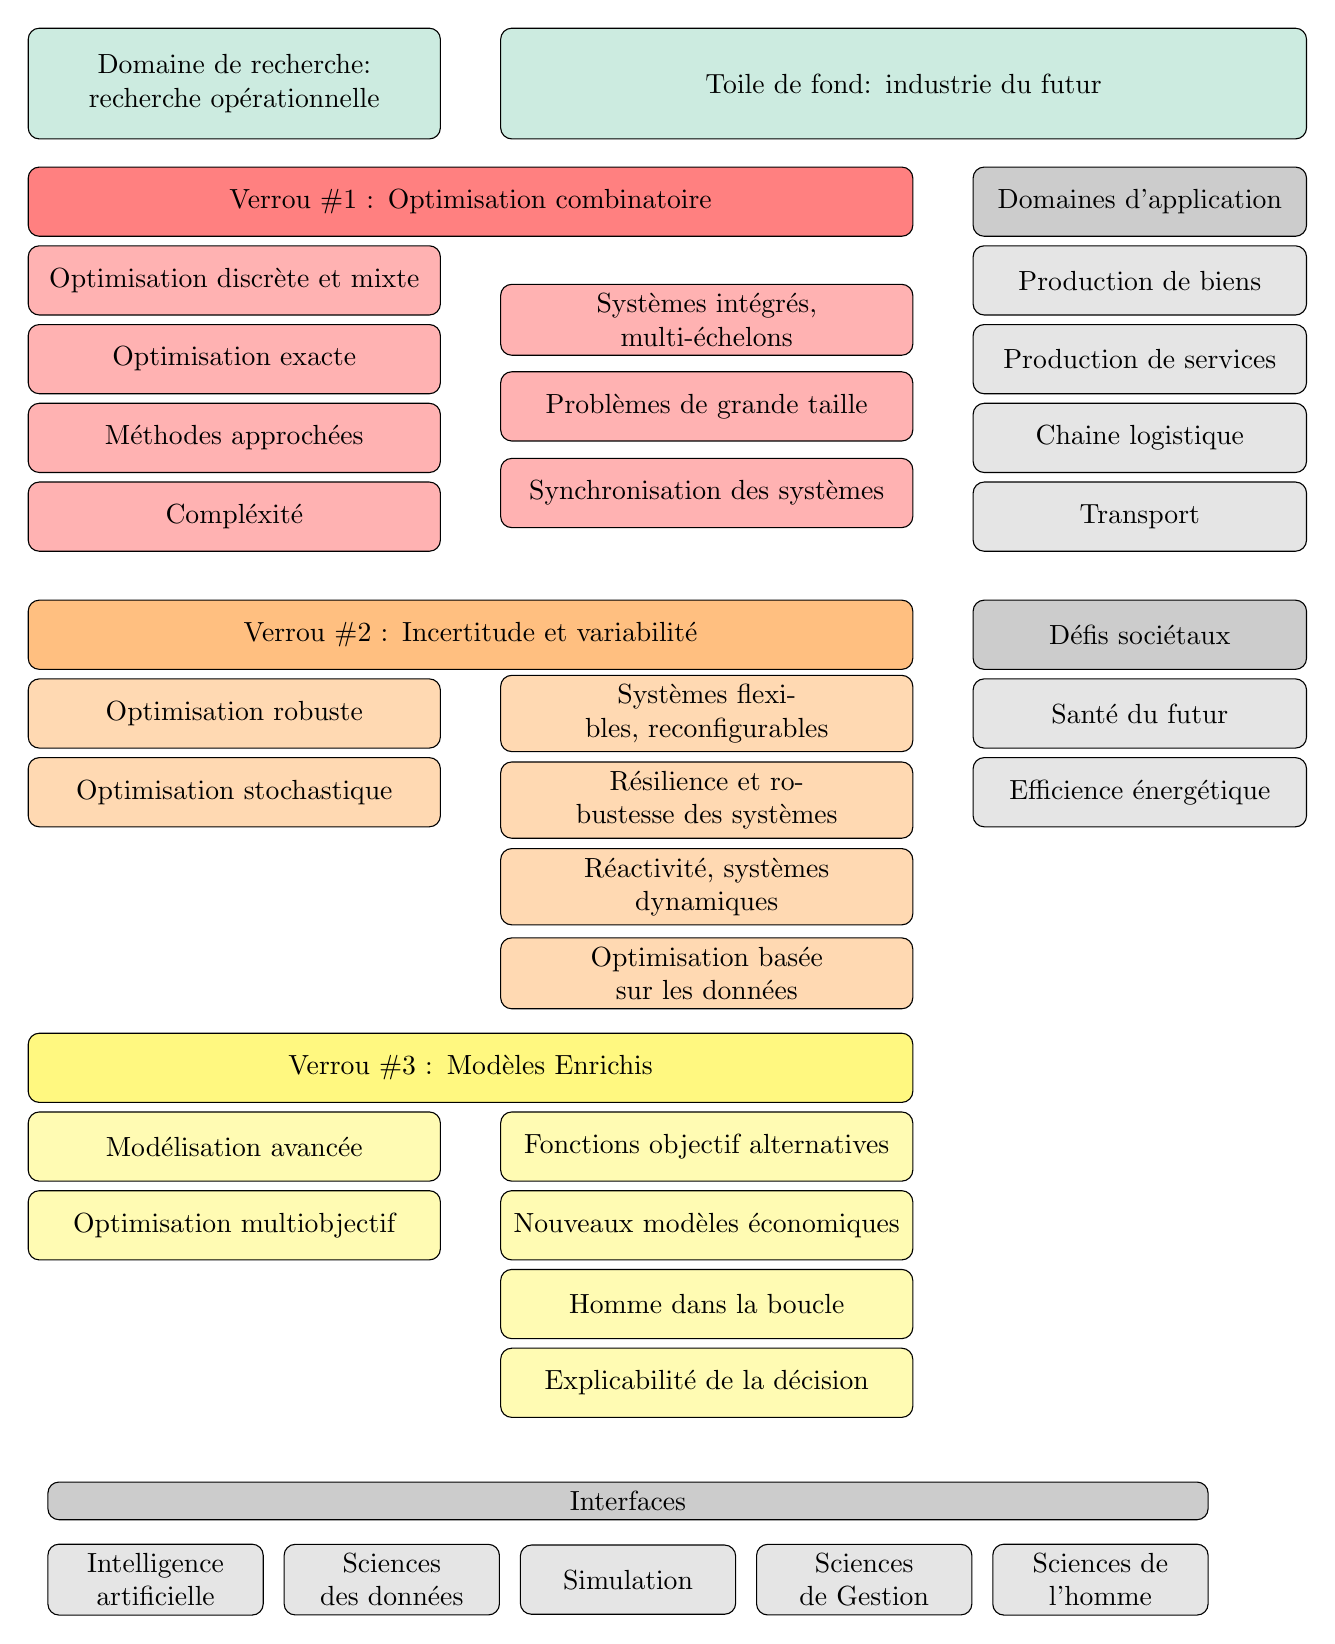
\begin{tikzpicture}[scale=0.5, auto]

    %  nodes  
    \node [chapeau, text width=5cm] (M) at (0,38) {Domaine de recherche: recherche opérationnelle};
    \node [chapeau, text width=10cm] (IF) at (17,38) {Toile de fond: industrie du futur};
    
         
   %-------------------------------------------------------------
     \node[verrou, fill=red!50] at (6,35) {Verrou \#1 : Optimisation combinatoire};
    \node[detail1] at (0,33) {Optimisation discrète et mixte};
    \node[detail1] at (0,31) {Optimisation exacte};
    \node[detail1] at (0,29) {Méthodes approchées};
    \node[detail1] at (0,27) {Compléxité};
    
   \node[detail1] at (12,32) {Systèmes intégrés, multi-échelons};
   \node[detail1] at (12,29.8) {Problèmes de grande taille};
   \node[detail1] at (12,27.6) {Synchronisation des systèmes};

    
    %-----------------------------------------------------------
   \node[verrou, fill = orange!50] at (6,24) {Verrou \#2 : Incertitude et variabilité};     
   \node[detail2] at (0,22) {Optimisation robuste};
    \node[detail2] at (0,20) {Optimisation stochastique};
    
    \node[detail2] at (12,22) {Systèmes flexibles, reconfigurables};
    \node[detail2] at (12,19.8) {Résilience et robustesse des systèmes};
    \node[detail2] at (12,17.6) {Réactivité, systèmes dynamiques};
    \node[detail2] at (12,15.4) {Optimisation basée sur les données};

  
  %---------------------------------------------------------
     \node[verrou, fill=yellow!50] at (6,13) {Verrou \#3 : Modèles Enrichis};

    \node[detail3] at (0,11) {Modélisation avancée};
    \node[detail3] at (0,9) {Optimisation multiobjectif};
    
    \node[detail3] at (12,11) {Fonctions objectif alternatives};
    \node[detail3] at (12,9) {Nouveaux modèles économiques};
    \node[detail3] at (12,7) {Homme dans la boucle};
    \node[detail3] at (12,5) {Explicabilité de la décision};
   
   
   %----------------------------------------------- 
   \node [detail, fill=gray!40] (D) at (23,35) {Domaines d'application};
    \node[detail] at (23,33) {Production de biens};
    \node[detail] at (23,31) {Production de services};
    \node[detail] at (23,29) {Chaine logistique};
    \node[detail] at (23,27) {Transport};

   \node [detail, fill=gray!40] (D) at (23,24) {Défis sociétaux};
    \node[detail] at (23,22) {Santé du futur};
    \node[detail] at (23,20) {Efficience énergétique};

     \node [chapeau2, text width=14.5cm] (I) at (10,2){Interfaces};
    \node[detail4] at (-2,0) {Intelligence artificielle};
    \node[detail4] at (4,0) {Sciences des données};
    \node[detail4] at (10,0) {Simulation};
    \node[detail4] at (16,0) {Sciences de Gestion};
    \node[detail4] at (22,0) {Sciences de l'homme};
    



  \end{tikzpicture}
  \caption{Détail du projet d'équipe}
  \end{figure}
  
  
		
		
		
		
		
		 
